Бутстреп - это компьютерный метод определения точности статистических оценок. Основная идея, лежащая в основе бутстрепа, очень проста и насчитывает как минимум два столетия. После ознакомления с некоторыми справочными материалами в этом отчете описывается метод бутстрепа и его применение для решения некоторых реальных задач анализа данных. В этой главе, помимо предварительного ознакомления с бутстрепом, рассматриваются некоторые фундаментальные идеи статистики. Основное внимание уделяется одному примеру статистики, для оценки точности котрой не нужен компьютер: выборочное среднее. Начнем с простого примера, касающегося средних и их расчетной точности. 

В таблице 2.1 показаны результаты небольшого эксперимента, в котором 7 из 16 мышей были случайным образом выбраны для получения нового лечения, а остальные 9 были отнесены к группе без лечения (контрольной). Лечение было направлено на продление выживаемости после тестовой операции. В таблице показано время выживания после операции в днях для всех 16 мышей. \newline

\noindent
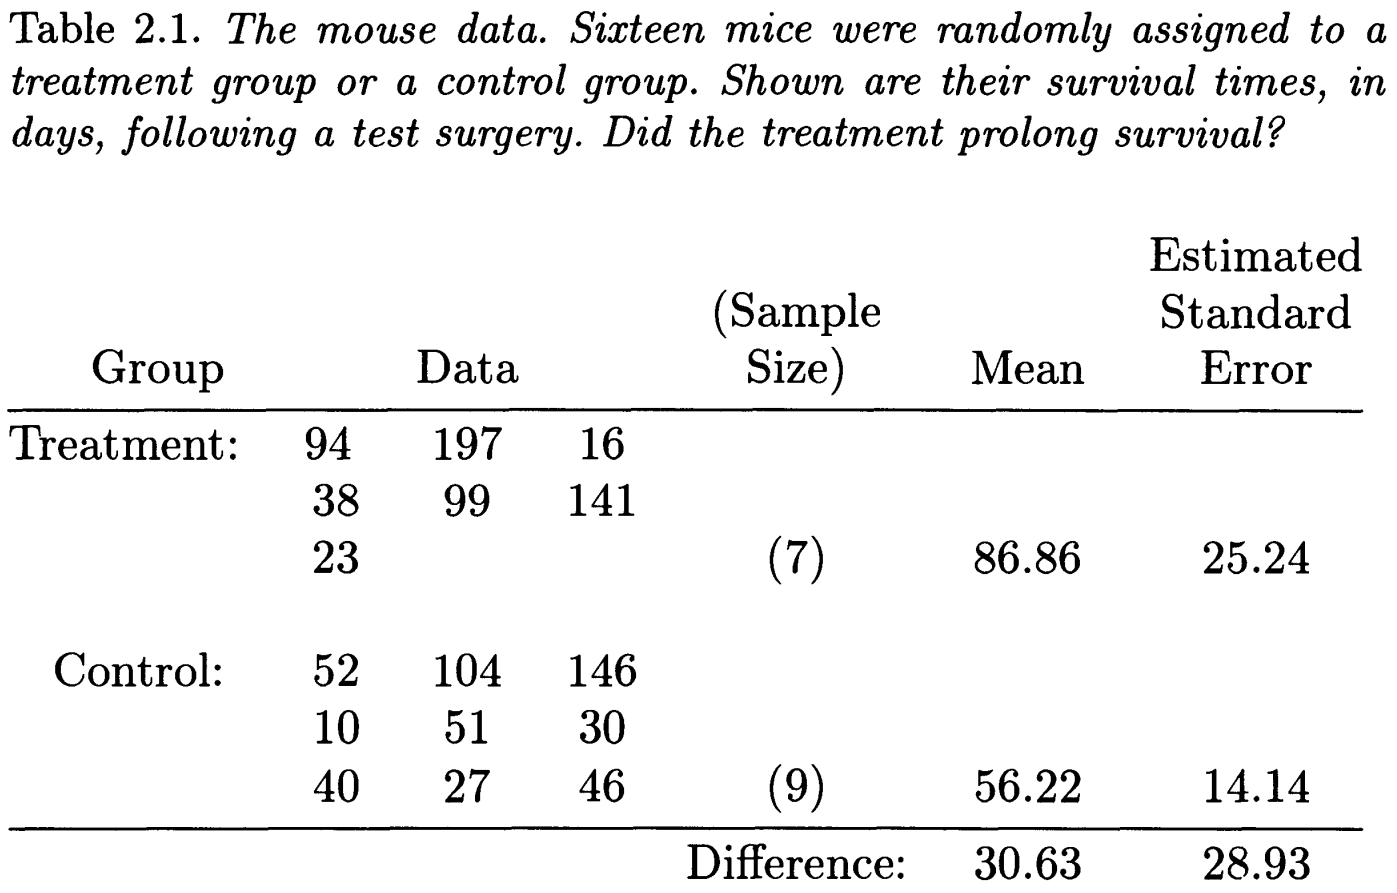
\includegraphics[width=\linewidth]{1/t1.png}
\newline

Продлило ли лечение выживаемость? Сравнение средних значений для двух групп дает предварительные основания для положительного ответа. Обозначим через $x_1,x_2,\ldots x_7$ продолжительность жизни в группе с лечением, соотв. $x_1=94,x_2=197,\ldots,x_7=23$, а через $y_1,y_2,\ldots y_9$ продолжительность жизни в контрольной группе. Групповые выборочные средние равны
\begin{equation}
    \overline x = \sum_{i=1}^7 x_i/7 = 86.86 \quad \texttt{и} \quad \overline y = \sum_{i=1}^9 y_i/9 = 56.22,
\end{equation}
таким образом разность $\overline x - \overline y$ равна $30.63$, что предполагает значительный эффект продления жизни при лечении.

Но насколько точны эти оценки? В конце концов, средние (2.1) основаны на небольших выборках, всего 7 и 9 мышей соответственно. Чтобы ответить на этот вопрос, нам нужна оценка точности выборочных средних $\overline x$ и $\overline y$). Для выборочных средних и по существу только для выборочных средних формулу точности получить легко. 

Расчетная стандартная ошибка среднего $\overline x$ на основе $n$ независимых наблюдений $x_1, x_2,\ldots, x_n$, $\overline x =\sum_{i=1}^n x_i/n$, определяется формулой 
\begin{equation}
    \sqrt{\frac{s^2}{n}},
\end{equation}
где $s^2=\sum_{i=1}^n (x_i-\overline x)^2/(n-1)$. (Эта формула и стандартные ошибки в целом обсуждаются более подробно в главе 4.) Стандартная ошибка любой оценки определяется как квадратный корень из ее дисперсии, то есть среднеквадратичная изменчивость оценки вокруг ее математического ожидания. Это наиболее распространенная мера точности оценок. Грубо говоря, оценка отличается от своего истинного значения менее чем на одну стандартную ошибку примерно в 68\% случаев и менее чем на две стандартные ошибки примерно в 95\% случаев.

Если бы оценочные стандартные ошибки в эксперименте на мышах были очень малы, скажем, менее 1, тогда мы бы знали, что $\overline x$ и $\overline y$ были близки к их истинным значениям и что наблюдаемая разница в 30,63, вероятно, была хорошей оценкой истинного увеличения выживаемости при лечении. С другой стороны, если формула (2.2) дает большие оценочные стандартные ошибки, скажем 50, тогда оценка разности будет слишком неточной, чтобы на нее можно было полагаться. 

Фактическая ситуация показана справа в Таблице 2.1. Расчетные стандартные ошибки, рассчитанные по (2.2), составляют 25,24 для $\overline x$ и 14,14 для $\overline y$. Стандартная ошибка для разности $\overline x - \overline y$ равна $28,93 = \sqrt{25,24^2 + 14,14^2}$ (поскольку дисперсия разности двух независимых величин является суммой их дисперсий). Мы видим, что наблюдаемая разница 30,63 составляет всего $30,63 / 28,93 = 1,05$ стандартной ошибки разности. Читатели, знакомые с теорией проверки гипотез, сочтут это незначимым результатом, который может легко возникнуть случайно, даже если лечение действительно не имело никакого эффекта. 

Обычно стандартные ошибки являются отличным первым шагом к критическому осмыслению статистических оценок. К сожалению, стандартные ошибки имеют серьезный недостаток: для большинства статистических оценок, отличных от среднего, не существует формулы, подобной (2.2), для получения стандартных ошибок. Другими словами, трудно оценить точность оценки, отличной от оценки среднего.

Предположим, например, что мы хотим сравнить две группы в таблице 2.1 по их медианам, а не по их средним значениям. Медианы составляют 94 для лечения и 46 для контроля, что дает разницу в 48, что значительно больше, чем разница средних значений. Но насколько точны эти медианы? Ответы на такие вопросы - вот где вступают в игру бутстреп и другие компьютерные методы. В оставшейся части этой главы дается краткий обзор начальной оценки стандартной ошибки - метода, который будет полностью обсуждаться в следующих главах. 

Предположим, что мы наблюдаем независимые данные $x_1, x_2,\ldots, x_n$, для удобства обозначенные вектором $X = (x_1, x_2, \ldots, x_n)$, по которым мы вычисляем интересующую статистику $s(X)$. Например, данные могут быть наблюдениями контрольной группы $n = 9$ в таблице 2.1, а $s(X)$ может быть средним по выборке. 

Бутстреп оценка стандартной ошибки, изобретенная Эфроном в 1979 году, выглядит совершенно иначе, чем (2.2), но на самом деле они тесно связаны. Бутстреп выборка $X^* = (x^*_i, x^*_2,\ldots, x^*_n)$ получается путем случайного выбора с возвращением $n$ точек из исходных данных $x_1, x_2,\ldots, x_n$. Например, при $n = 7$ мы можем получить $X^* = (x_5, x_7, x_5, x_4, x_7, x_3, x_1)$· 
\newline

\noindent
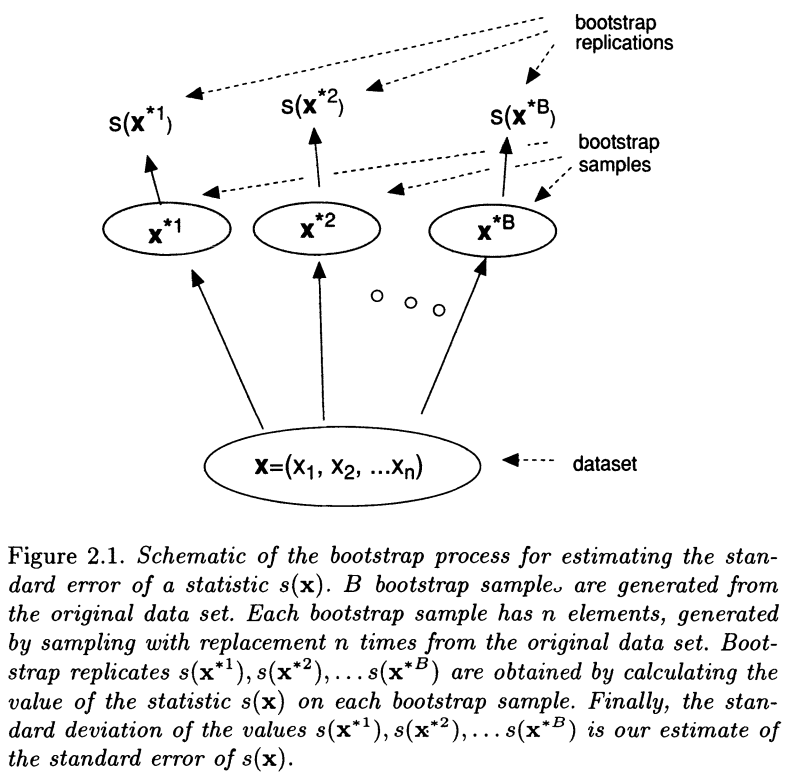
\includegraphics[width=\linewidth]{1/f1.png}
\newline

Рисунок 2.1 представляет собой схему процесса бутстрепа. Алгоритм бутстрепа начинается с генерации большого количества независимых бутстреп выборок $X^{*1}, X^{* 2},\ldots, X^{*B}$, каждая размером n. Типичные значения для B, количества бутстреп выборок, находятся в диапазоне от 50 до 200 для оценки стандартной ошибки. Каждой бутстреп выборке соответствует бутстреп репликация $s (X^{* b})$, посчитанная для $X^{* b}$. Если $s(X)$ - это, например, медиана выборки, то $s (X^*)$ - это медиана бутстреп выборки. Бутстреп оценка стандартной ошибки - это стандартное отклонение бутстреп репликаций  
\begin{equation}
    \hat{se}_{boot}=\left\{\sum_{b=1}^B [s(X^{*b})-s(\cdot)]^2/(B-1)\right\}^{\frac{1}{2}},
\end{equation}
где $s(\cdot)=\sum_{b=1}^B s(X^{*b})/B$. Предположим, что $s(X)=\overline X$. В этом случае стандартная теория вероятностей говорит нам, что, когда B становится очень большим, формула (2.3) приближается к  
\begin{equation}
    \left\{\sum_{i=1}^n (x_i-\overline x)^2/n^2\right\}^{\frac{1}{2}}.
\end{equation}

Это почти то же самое, что и формула (2.2). Мы могли бы сделать это точно таким же, умножив определение (2.3) на множитель $[n / (n-1)] ^\frac{1}{2}$, но в этом нет практического смысла. 
\newline

\noindent
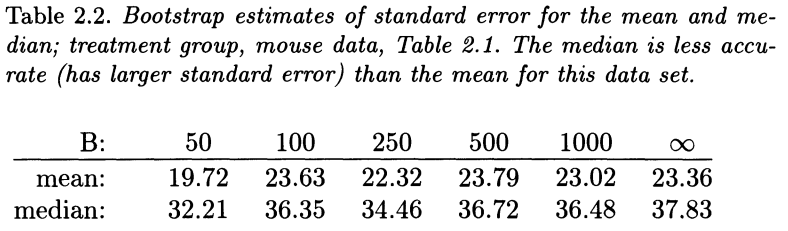
\includegraphics[width=\linewidth]{1/t2.png}
\newline

В таблице 2.2 показаны бутстрап оценки стандартной ошибки для среднего и медианы для данных экспериментальной группы мышей из таблицы 2.1. Стандартные ошибки уменьшаются до предельных значений по мере увеличения числа бутстраповых выборок $B$. Предельное значение $23,36$ для среднего получается из (2.4). Формула для предельного значения $37,83$ для стандартной ошибки медианы довольно сложна. 

Теперь мы можем оценить точность разницы медиан между двумя группами. Описанная выше бутстреп процедура, примененная к контрольной группе, дала оценку стандартной ошибки $11,54$ на основе $B = 100$ повторений ($B = \infty$ дало $9,73$). Следовательно, используя $B = 100$, наблюдаемая разница в $48$ имеет расчетную стандартную ошибку $\sqrt{36,35^2 + 11,54^2} = 38,14$, и, следовательно, $48 / 38,14 = 1,26$ стандартной ошибки. Это больше, чем наблюдаемая разница в средних, но все же незначимо. 

Для большинства статистических данных у нас нет формулы для предельного значения стандартной ошибки, но на самом деле формула не нужна. Вместо этого мы используем числовой вывод бутстреп программы для некоторого удобного значения B. Легко написать бутстреп программу, которая работает для любой вычислимой статистики $s (X)$. Имея эти программы, аналитик данных может свободно использовать любую статистику, независимо от ее сложности, с уверенностью, что он или она также будет иметь разумное представление о точности оценки. Применение бутстрепа стало доступным, поскольку компьютеры стали мощнее и дешевле. 
Стандартные ошибки - это простейшие меры статистической точности. В последующих главах показано, как бутстреп методы могут оценивать более сложные меры точности, такие как смещения, ошибки прогнозирования и доверительные интервалы. Бутстрепированные доверительные интервалы увеличивают вычислительную нагрузку еще в 10 раз. Результатом всех этих вычислений является увеличение количества статистических проблем, которые могут быть проанализированы, сокращение допущений анализа и устранение рутинных, но утомительных теоретических расчетов, обычно связанных с оценкой точности. 